\documentclass[a4j,dvipdfmx]{jsarticle}
\usepackage{amsmath,amssymb}
\usepackage{siunitx}
\usepackage{ascmac}
\usepackage[dvips]{graphicx}
\usepackage{listings}

\renewcommand{\thesection}{\Roman{section}}
\renewcommand{\thesubsection}{\roman{subsection}}
\begin{document}
\part*{多重積分}
\section{多重積分}
\subsection{二重積分}
一変数の関数$y=f(x)$の定積分$\displaystyle \int_a^b f(x)dx$は去年学んだ。
少しだけ復習すると、積和の極限、すなわち$\displaystyle \lim_{n\to\infty}\sum_{k=1}^{n}f(\zeta_k)\Delta x_k$が定積分であった。これから、定積分を二変数の場合に拡張する。いままでは、積分領域は線分であったが、
今度は積分領域が面になる。

$xy$平面の領域$R$で定義された連続な関数を$f(x,y)$とする。領域$R$を、各々の面積が$\Delta A_1,\Delta A_2,\cdots,\Delta A_n$の
$n$個の章領域$R_1,R_2,\cdots,R_n$に分割する。小領域$R_1$内に点$P_1(\zeta_1,\eta_1)$、小領域$R_2$内に
$P_2(\zeta_2,\eta_2),\cdots,R_n$内に点$P_n(\zeta_n,\eta_n)$を選び、積和の極限
\begin{equation}
    \sum_{k=1}^{n}f(P_k)\Delta A_k=\sum_{k=1}^{n}f(\zeta_k,\eta_k)\Delta A_k\label{6.2}
\end{equation}
を作る。各小領域の直径(領域内のに転換の距離の最大値)が0に近づくように分割を細かくしていく。この時の極限値を
\begin{equation}
    \iint_R f(x,y)dA=\lim_{n\to\infty}\sum_{k=1}^{n}f(\zeta_k.\eta_k)\Delta A_k\label{6.3}
\end{equation}
とかき、関数$f(x,y)$の領域$R$における\textbf{二重積分}という。積分記号が二つあるのは、二変数関数の定積分であることを
示し、積分記号の添え字$R$は$x,y$の値の領域を表している。

特に、$f(x,y)=1$と置けば、その二重積分は領域$R$の面積$A$を与える。すなわち、
\begin{equation}
    A=\iint_RdA\label{6.4}
\end{equation}
\subsection{二重積分と体積}
定積分が面積と関係していたように、二重積分\eqref{6.3}式は体積と関係している。関数$z=f(x,y)$は領域
$R$で正とする。積和\eqref{6.2}の各項$f(\zeta_k,\eta_k)\Delta A_k$は、高さが$z_k=f(\zeta_k,\eta_k)$で、上下の平行面の面積が$\Delta A_k$の
垂直な``柱"の体積を与える。これは、底面積が$\Delta A_k$で、上面が曲線$z=f(x,y)$で与えられる垂直な柱の体積
を近似したものである。すなわち、\eqref{6.2}の積和は、局面下の体積を近似している。こうして、この極限値である二重積分\eqref{6.3}は、
局面$z=f(x,y)$、底面$R$、$R$の周上に建てた垂直面、がつくる領域の体積に等しいことがわかる。
\subsection{三重積分}
二重積分を導入したのと同じようにして、三重積分が定義される。三次元の領域$R$で連続な関数$f(x,y,z)$を考える。
領域$R$を、各体積が$\Delta V_1,\Delta V_2,\cdots,\Delta V_n$である$n$個の小区間$R_1,R_2,\cdots,R_n$に分割する。
小領域$R_k$内に点$P_k(\zeta_k,\eta_k,\xi_k)$をとり、積和
\begin{equation}
    \sum_{k=1}^{n}f(P_k)\Delta V_k=\sum_{k=1}^{n}f(\zeta_k,\eta_k,\xi_k)\Delta V_k\label{6.5}
\end{equation}
を作る。各小領域$R_k$の直径を0にするように、分割の数$n$を大きくする。その極限値を
\begin{equation}
    \iiint_R f(x,y,z)dV=\lim_{n\to\infty}\sum_{k=1}^{n}f(\zeta_k,\eta_k,\xi_k)\Delta V_k\label{6.6}
\end{equation}
と書き、領域$R$での関数$f(x,y,z)$の\textbf{三重積分}という。特に$f(x,y,z)=1$ならば、
三重積分は領域$R$の体積$V$を与える。すなわち、
\begin{equation}
    V=\iiint_R dV\label{6.7}
\end{equation}

同様にして、$n$次元での領域$R$で連続な関数$f(x_1,x_2,\cdots,x_n)$に対して、$n$重積分が定義される。

二重積分や三重積分を、\eqref{6.3}や\eqref{6.6}式のように積和の極限として計算するのはすごく面倒だ。
そこで実際には定積分と同様に、もっと楽に計算をする。そのための方法を次節で紹介する。

\section{二重積分は積分を2度行う}
\subsection{累次積分}
まず二重積分について考える。積分領域$R$の境界は、$x$軸または$y$軸に平行な線と3回以上交わらないとしよう。(下図参照)
\begin{figure}[h]
    \centering
    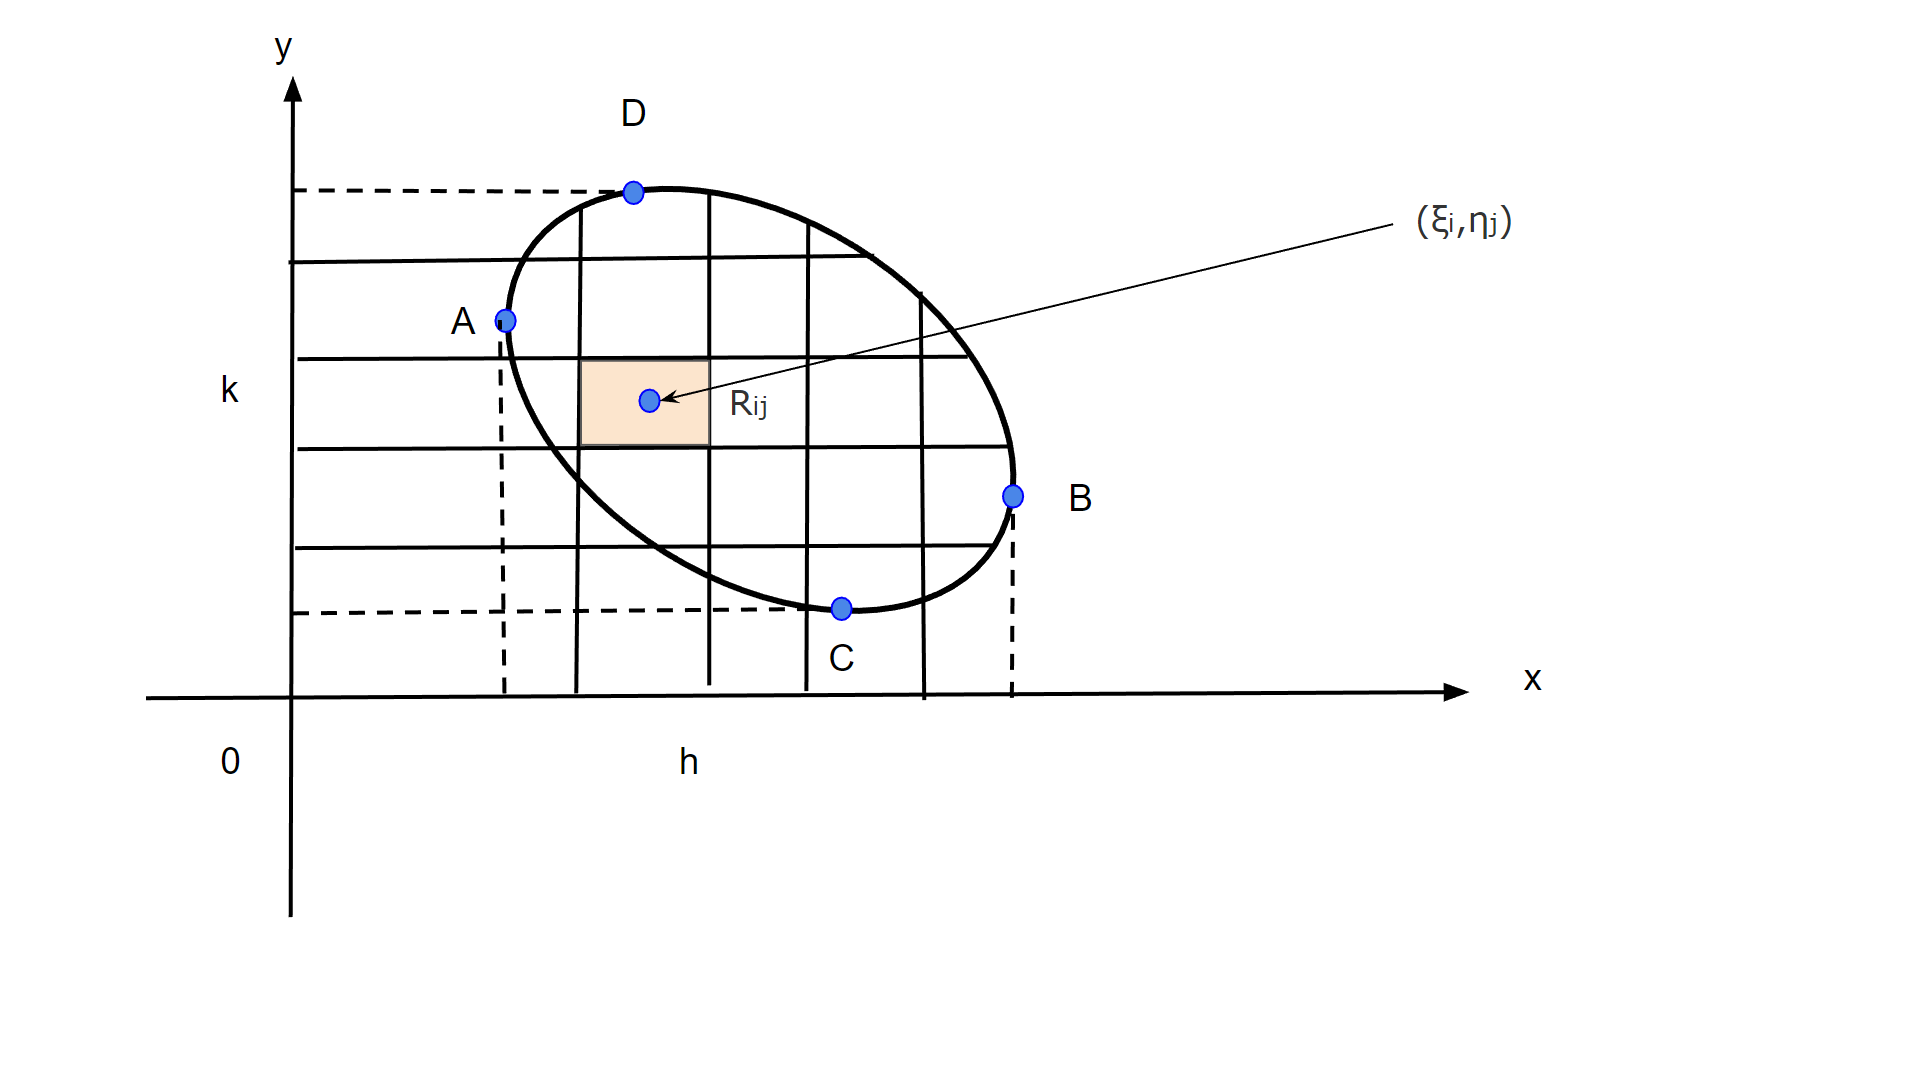
\includegraphics[width=10cm,scale=5]{img/累次積分.png}
    \caption{累次積分}
\end{figure}

より複雑な形の領域は、このような領域に分けられる。曲線ACBを$y=g(x)$,曲線BDAを$y=h(x)$
で表す。

区間$a\leq x\leq b$を、長さが$\Delta x_1,\Delta x_2,\cdots,\Delta x_m$の$m$個の小区間
$h_1,h_2.\cdots,h_m$に分割する。また、区間$c\leq y\leq d$を、長さが$\Delta y_1,\Delta y_2,\cdots,\Delta y_n$の$n$個の小区間
$k_1,k_2,\cdots,k_n$に分割する。そして、直線$x=x_1,x=x_2,\cdots,x=x_{m+1},y=y_1,y=y_2,\cdots,y=y_{n+1}$を引くと、領域$R$は
各面積が$\Delta x_i\Delta y_j$の長方形の領域$R_{ij}$に分割される。境界の近くでは長方形にはならないが、$m,n$が大きい限り、それらの寄与は無視できる。
領域$R_{ij}(i=1,2,\cdots,m,j=1,2,\cdots,n)$は全部で$mn$個ある。領域$R_{ij}$内に点$(\xi_i,\eta_j)$を選び、積和
\begin{equation}
    \sum_{i=1}^{m}\sum_{j=1}^{n}f(\xi_i,\eta_j)\Delta x_i\Delta y_j\label{6.8}
\end{equation}
を作る。

これは、\eqref{6.2}式の特別な場合であることに注意しよう。各区間の長さが0になるように、$m,n$を大きくすれば、
二重積分\eqref{6.3}式に等しい。

いま、最初に区間$h_i$を固定し、その上に並んだ長方形をおいて、積和
\begin{equation}
    \left\{\sum_{j=1}^{n}f(\xi_i,\eta_j)\Delta y_j\right\}\Delta x_i\quad(i\text{は固定})\label{6.9}
\end{equation}
を考える。そして、$y$軸方向の区間$k_j$の長さが0になるように$n\to\infty$の極限を取ると、
\begin{equation}
    \lim_{n\to\infty} \left\{\sum_{j=1}^{n}f(\xi_i,\eta_j)\Delta y_j\right\}\Delta x_i=\left\{\int_{g(\xi_i)}^{h(\xi_i)}f(\xi_i,\eta_j)dy\right\}\Delta x_i\label{6.10}
\end{equation}
を得る。次に、x軸方向の区間に対して和を取り、$m\to\infty$の極限を取ると
\begin{equation}
    \lim_{m\to\infty}\sum_{i=1}^{m}\left\{\int_{g(\xi_i)}^{h(\xi_i)}f(\xi_i,\eta_j)dy\right\}\Delta x_i=\int_a^b\left[\int_{g(\xi_i)}^{h(\xi_i)}f(\xi_i,\eta_j)dy\right]dx\label{6.11}
\end{equation}
が得られる。こうして、二重積分は、$f(x,y)$の$y$についての積分を行い、次に$x$についての積分を行うことで計算できることがわかる。
また、これは$x$積分と$y$積分の順序を入れ替えても同じである。

積分\eqref{6.11}式を\textbf{累次積分}という。

以上まとめるなら、$f(x,y)$が領域$R$で連続ならば、
\begin{align}
    \iint_R f(x,y)dxdy&=\int_a^b\int_{g(x)}^{h(x)}f(x,y)dydx\notag\\
    &=\int_c^d\int_{k(y)}^{l(y)}f(x,y)dxdy\label{6.13}
\end{align}

\subsubsection*{例題}
次の積分を求めよ。
\begin{equation*}
    (1)\int_0^q\int_0^xdydx\qquad(2)\int_0^1\int_1^2(x+y)dxdy
\end{equation*}

\subsubsection*{解答}
\begin{align*}
    &(1)\int_0^1\int_0^xdydx=\int_0^1[y]_0^xdx=\int_0^1xdx=\frac{1}{2}\\
    &(2)\int_0^1\int_1^2(x+y)dxdy=\int_0^1\left[\frac{x^2}{2}+xy\right]_1^2dy=
    \int_0^1(\frac{3}{2}+y)dy=\frac{3}{2}+\frac{1}{2}=2
\end{align*}

\subsubsection*{例題}
直線$y=x,x=1,y=0$で囲まれた領域を$R$とするとき、次の二重積分を求めよ。
\begin{equation*}
    I=\iint_R(x^2+y^2)dxdy
\end{equation*}

\subsubsection*{解答}
最初に、$y$積分、$x$積分の順に計算する。
\begin{equation*}
    I=\int_0^1\left\{\int_0^x (x^2+y^2)dy\right\}dx=\frac{1}{3}
\end{equation*}
次に、$x$積分、$y$積分の順に計算する。
\begin{equation*}
    I=\int_0^1\left\{\int_y^1(x^2+y^2)dx\right\}dy=\frac{1}{3}
\end{equation*}
\subsubsection*{}
三重積分の場合にも、同様に累次積分が定義される。
\begin{equation}
    \iiint_R f(x,y,z)dxdydz=\int_a^b\left[\int_{y_1(x)}^{y_2(x)}\left\{\int_{z_1(x,y)}^{z_2(x,y)}f(x,y,z)dz\right\}dy\right]dx\label{6.14}
\end{equation}
上の式では、積分はかっこの内側から順に行う。すなわち$x,y$を固定して、$z$積分を行い、次に$x$を固定して
$y$積分を行い、最後に$x$積分を行う。二重積分と同様に、$f(x,y,z)$が連続ならば、個の積分は存在して、積分の
順序を変えることができる。

\subsubsection*{例題}
\begin{equation*}
    I=\int_0^1\int_0^{1-x}\int_0^{2-y}xyzdzdydx
\end{equation*}
を求めよ。

\subsubsection*{解答}
\begin{align*}
    I&=\int_0^1\int_0^{1-x}\int_0^{2-y}xyzdzdydx\\
     &=\int_0^1\int_0^{1-x}\frac{xy}{2}(2-y)^2dydx\\
     &=\int_0^1\frac{1}{2}x\left\{\frac{1}{4}(1-x)^4-\frac{4}{3}(1-x)^3+2(1-x)^2\right\}dx\\
     &=\int_0^1\frac{1}{2}\left(\frac{1}{4}x^5+\frac{1}{3}x^4-\frac{1}{2}x^3-x^2+\frac{11}{12}x\right)dx=\frac{13}{240}
\end{align*}

\section{積分変数の変換}
\subsection{座標系}
まず始めに、直交座標での多重積分をまとめる。

二重積分は、直交座標$(x,y)$において、
\begin{equation}
    \iint_R f(x,y)dxdy\label{6.15}
\end{equation}
で与えられる。$dA=dxdy$を直交座標での\textbf{面積要素}という。

また、三重積分は、直交座標$(x,y,z)$において、
\begin{equation}
    \iiint_R f(x,y,z)dxdydz\label{6.16}
\end{equation}
で与えられる。$dV=dxdydz$を直交座標での\textbf{体積要素}という。

これらの多重積分を実行する際は、積分領域の形によっては、直交座標系よりはほかの座標系を用いたほうが簡単になること
がある。また、応用上では、問題設定の初めからほかの座標系を使って議論することも多い。
よく用いられる座標系に対して、多重積分がどのように定義されるかを調べてみよう。
\subsection{2次元極座標}
2次元極座標$(\rho ,\phi)$は、直交座標$(x,y)$を用いて
\begin{align}
    x=\rho\cos\phi,\quad y=\rho\sin\phi\label{6.17}\\
    (0\leq\rho\leq\infty,0\leq\phi\leq2\pi)\notag
\end{align}
または、
\begin{equation}
    \rho=\sqrt{x^2+y^2},\quad\phi=\arctan\frac{y}{x}\label{6.18}
\end{equation}
で定義される。\eqref{6.17}式と\eqref{6.18}式は同じことを意味していることに気づけるだろうか。
$\rho=$一定の曲線は原点を中心とする円であり、$\phi=$一定は原点を通る半直線である。
半径が$\rho,\rho+\Delta\rho$の2つの同心円と、角$\phi,\phi+\Delta\phi$の2つの半直線とで
囲まれる領域を考える。この領域は、$\Delta \rho$と$\Delta\phi$が十分小さいならば、辺の長さが
$\Delta\rho,\rho\Delta\phi$の長方形とみなすことができるので、その面積$\Delta A$は、
\begin{equation}
    \Delta A=\rho\Delta\phi\cdot\Delta\rho=\rho\Delta\rho\Delta\phi\label{6.19}
\end{equation}
で与えられる。したがって、2次元座標系での二重積分は、
\begin{equation}
    \lim_{n\to\infty}\sum_{k=1}^{n}f(P_k)\Delta A_k=\iint_Df(\rho\cos\phi,\rho\sin\phi)\rho d\rho d\phi\label{6.20}
\end{equation}
となる。領域$D$は直交座標での領域を2次元極座標で表したものである。

\subsubsection*{例題}
次の積分を求めよ。
\begin{equation*}
    I=\iint_R e^{-(x^2+y^2)}dxdy\quad(R:0\leq x^2+y^2\leq a^2)
\end{equation*}

\subsubsection*{解答}
$x=\rho\cos\phi,y=\rho\sin\phi$遠く。領域$R$は、$0\leq\rho\leq a,0\leq\phi\leq 2\pi$
に変換される。また、$x^2+y^2=\rho^2$である。よって、\eqref{6.20}式より、
\begin{equation*}
    I=\int_0^{2\pi}\int_0^ae^{-\rho^2}\rho d\rho d\phi=2\pi\int_0^a e^{-\rho^2}\rho d\rho
    =\pi(1-e^{-a^2})
\end{equation*}

さて、この時、$a\to\infty$としてみると、$x,y$の積分領域は、各々独立に$-\infty$から$+\infty$になるから、
\begin{equation*}
    I=\int_{-\infty}^{\infty}\int_{-\infty}^{\infty} e^{-(x^2+y^2)}dxdy=\left\{\int_{-\infty}^{\infty}e^{-x^2}dx\right\}^2
    =\lim_{a\to\infty}\pi(1-e^{-a^2})=\pi
\end{equation*}
よって、
\begin{equation}
    \int_{-\infty}^{\infty}e^{-x^2}dx=\sqrt{\pi}\label{6.21}
\end{equation}
を得る。これは有名な\textbf{ガウス積分}であり、確率論や統計力学で非常によく用いられる。

\subsection{極座標}
極座標$(r,\theta,\phi)$は、直交座標$(x,y,z)$を用いて、次のように表せる。
\begin{align}
    x=r\sin\theta\cos\phi,\quad y=r\sin\theta\sin\phi,\quad z=r\cos\theta\notag\\
    (0\leq r\leq\infty,\quad 0\leq\theta\leq\pi,\quad 0\leq\phi\leq 2\pi)\label{6.25}
\end{align}
で定義される。任意の点を$P$とするとき、線分OPの長さが$r$、$z$軸と線分OPのなす角は$\theta$、
軸O$z$と点Pを通る半平面が平面$xOz$となす角は$\phi$である。当然のことながら、$\displaystyle\theta=\frac{\pi}{2}$
と置けば、二次元極座標と同じである。
\begin{figure}[h]
    \centering
    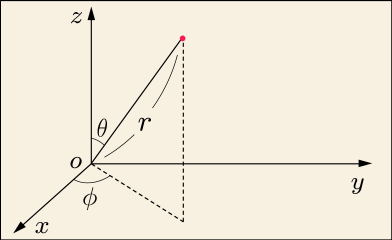
\includegraphics[width=10cm,scale=5]{img/calculus4c.png}
    \caption{極座標(引用:https://eman-physics.net/math/calculus04.html )}
\end{figure}

$r=$一定は原点Oを中心とする球面を表す。$\theta =$一定は$z$軸を回転軸とする円錐面を与える。
また,$\phi =$一定は、$z$軸を通る半平面平面を表す。いま、半径が、$r,r+\Delta r$の二つの
同心球、頂角が$\theta ,\theta+\Delta \theta$の二つの円錐面、$\phi,\phi+\Delta\phi$の二つの半平面、で
囲まれる領域を考える。
この領域は、$\Delta r,\Delta \phi,\Delta\theta$が十分小さいならば、辺の長さ$\Delta r,r\Delta\theta,r\sin\theta\Delta \phi$
の直方体とみなすことができるので、その体積は$\Delta V$は、
\begin{equation}
    \Delta V=\Delta r\cdot r\Delta\theta\cdot r\sin\theta\Delta\phi=r^2\sin\theta\Delta r\Delta\theta\Delta\phi\label{6.26}
\end{equation}
で与えられる。したがって、極座標系での三重積分は、
\begin{equation}
    \lim_{n\to\infty}\sum_{k=1}^{n}f(P_k)\Delta V_k=\iiint_D f(r\sin\theta\cos\phi,r\sin\theta\sin\phi,r\cos\theta)r^2\theta drd\theta d\phi\label{6.27}
\end{equation}
となる。領域Dは、直角座標$(x,y,z)$での領域を極座標で表したものであり、また、$r^2\sin\theta drd\theta d\phi$は極座標での体積要素である。
\subsubsection*{例題}
次の三重積分を求めよ。
\begin{equation*}
    I=\iiint_R(x^2+y^2+z^2)dxdydz\quad(R:0\leq x^2+y^2+z^2\leq a^2,a>0)
\end{equation*}
極座標変換すると、簡単に求まる。$x^2+y^2+z^2=r^2$に注意して、
\begin{equation*}
    I=\int_0^{2\pi}d\phi\int_0^\pi d\theta\int_0^a r^2\cdot r^2\sin\theta dr
    =2\pi\cdot\frac{1}{5}a^5\cdot 2=\frac{4\pi}{5}a^5
\end{equation*}
となる。
\subsubsection*{}
\subsection{曲線座標}
もっと一般に、
\begin{equation*}
    x=g(u,v),\quad y=h(u,v)
\end{equation*}
で与えられる曲線座標系$(u,v)$では、二重積分はどう表せるのか考えてみよう。
結論だけ与えると、二重積分は
\begin{align}
    \iint_R f(x,y)dxdy=\iint_D f(g(u,v),h(u,v))|J|du dv\notag\\
    J=\frac{\partial(x,y)}{\partial(u,v)}=
    \begin{vmatrix}
        \displaystyle\frac{\partial x}{\partial u} & \displaystyle\frac{\partial x}{\partial v}\\
        &\\
        \displaystyle\frac{\partial y}{\partial u} & \displaystyle\frac{\partial y}{\partial v}
    \end{vmatrix}
    =\frac{\partial x}{\partial u}\frac{\partial y}{\partial v}-\frac{\partial x}{\partial u}\frac{\partial y}{\partial v}\label{6.33}
\end{align}
となる。ここで、$J$は$u,v$に関する$x,y$の\textbf{ヤコビ行列式}または、\textbf{ヤコビアン}という。
$|J|$は、その絶対値である。

\subsubsection*{例題}
二次元極座標$(\rho,\phi)$に対して、
\begin{equation*}
    \iint_R f(x,y)dxdy=\iint_Df(\rho\cos\phi,\rho\sin\phi)\rho d\rho d\phi
\end{equation*}
を示せ。

\subsubsection*{解答}
公式\eqref{6.33}式より、
\begin{equation*}
    J=\begin{vmatrix}
        \displaystyle\frac{\partial x}{\partial u} & \displaystyle\frac{\partial x}{\partial v}\\
        &\\
        \displaystyle\frac{\partial y}{\partial u} & \displaystyle\frac{\partial y}{\partial v}
    \end{vmatrix}
    =\begin{vmatrix}
        \cos\phi & -\rho\sin\phi\\
        &\\
        \sin\phi & \rho\cos\phi
    \end{vmatrix}
    =\cos\phi\cdot\rho\cos\phi - (-\rho\sin\phi)\sin\phi=\rho(\sin^2\phi+\cos^2\phi)=\rho
\end{equation*}
よって、$xy$座標系での領域$R$を$uv$座標系で表した領域を$D$として、
\begin{equation*}
    \iint_R f(x,y)dxdy=\iint_Df(\rho\cos\phi,\rho\sin\phi)\rho d\rho d\phi
\end{equation*}
を得る。

\section{線積分}
\subsection{線積分}
この章の最後の課題として、線積分について述べる。理工学でよく用いられる概念らしい。

ひとまず定義から述べる。三次元空間内に、方向を持った曲線$C$を考える。その$C$上のすべての点において連続な関数
$P(x,y,z),Q(x,y,z),R(x,y,z)$があるとする。

いま、曲線$C$上に$n-1$個の点$(x_1,y_1,z_1),(x_2,y_2,z_2),\cdots,(x_{n-1},y_{n-1},z_{n-1})$をとり、
$n$個の小区間に分ける。始点$A$を$(a_1,a_2,a_3)\equiv(x_0,y_0,z_0)$、終点$B$を$(b_1,b_2,b_3)\equiv(x_n,y_n,z_n)$
と書き、$\Delta x_k=x_k-x_{k-1},\Delta y_k=y_k-y_{k-1},\Delta z_k=z_k-x_{k-1}(k=1,2,\cdots,n)$と置く。
点$(x_{k-1},y_{k-1},z_{k-1})$と$(x_k,y_k,z_k)$の間の$C$上の点を$(\xi_k,\eta_k,\zeta_k)$として、積和
\begin{equation}
    \sum_{k=1}^{n}\{P(\xi_k,\eta_k,\zeta_k)\Delta x_k+Q(\xi_k,\eta_k,\zeta_k)\Delta y_k+R(\xi_k,\eta_k,\zeta_k)\Delta z_k\}\label{6.49}
\end{equation}
をつくる。すべての$\Delta x_k,\Delta y_k,\Delta z_k$が$0$に近づくように分割の数$n$を大きくする。
この時の極限値を
\begin{equation}
    \int_C[P(x,y,z)dx+Q(x,y,z)dy+R(x,y,z)dz]\label{6.50}
\end{equation}
で表し、\textbf{線積分}という。線積分は、一般に始点Aと終点Bをつなぐ曲線(\textbf{積分路})の選び方に依存する。
そのため、選んだ経路は$\int_C$のように選んだ積分路を積分記号の横に書く。

曲線Cが$xy$平面上の曲線である場合は、線積分は
\begin{equation*}
    \int_C[P(x,y)dx+Q(x,y)dy]
\end{equation*}
となる。

線積分の性質をまとめる。
\begin{itemize}
    \item $\displaystyle\int_C[Pdx+Qdy+Rdz]=\int_CPdx+\int_CQdy+\int_CRdz$
    \item 曲線$C$の逆向きの曲線を$\overline{C}$とする。\\
    \begin{equation*}
        \int_{\overline{C}}[Pdx+Qdy+Rdz]=-\int_C[Pdx+Qdy+Rdz]
    \end{equation*}
    \item 曲線$C_1,C_2$をつなぎ合わせた曲線を$C$とする。\\
    \begin{equation*}
        \int_C[Pdx+Qdy+Rdz]=\int_{C_1}[Pdx+Qdy+Rdz]+\int_{C_2}[Pdx+Qdy+Rdz]
    \end{equation*}
\end{itemize}

\subsubsection*{例題}
線積分
\begin{equation*}
    \int_C[(x-y)dx+ydy]
\end{equation*}
を次の二つの積分路で求めよ。\\
(1)$C_1:$x軸上を始点$(1,0)$から$(2,0)$。次にy軸に平行に$(2,0)$から終点$(2,1)$。\\
(2)$C_2:$始点$(1,0)$と終点$(2,1)$を結ぶ直線。

\subsubsection*{解答}
(1)求める線積分は
\begin{equation*}
    \int_1^2 xdx+\int_0^1 ydy=\frac{3}{2}+\frac{1}{2}=2
\end{equation*}
左辺第一項はx軸の線、第二項はy軸平行の直線を表す。

(2)始点と終点を結ぶ直線$C_2$は$y=x-1(1\leq x\leq 2)$であるため、$C_2$上では$dy=dx$となる。
よって、
\begin{equation*}
    \int_{C_2}[(x-y)dx+ydy]=\int_1^2[(x-(x-1))dx+(x-1)dx]=\int_1^2 xdx=\frac{3}{2}
\end{equation*}
この答えから、始点終点が共通でも、積分路が異なると、線積分の値が異なることに注意しよう。

\subsection{仕事}
線積分は、力学の仕事をイメージすると理解しやすいかもしれない。位置に依存して働く力の$x,y,z$成分をそれぞれ$P,Q,R$とすれば、
$Pdx,Qdy,Rdz$は微小区間におけるそれぞれの方向の仕事($=\text{力}\times\text{変位}$)になることがわかるだろうか。
線積分はそれらの総和であるわけだから、全体の仕事となるわけである。
\subsection{重力による位置エネルギー}
物理の授業では、重力による位置エネルギー(ポテンシャルエネルギー)は$U=mgh$で与えられることを学んだ。
この式から、重力による位置エネルギーは途中の経路によらず、物体の位置によって決まるということがわかる。
この理由を、線積分をつかって考えてみよう。

まず、選んだ経路を$C$とすると、重力による位置エネルギー$U$は次のように表せる。
\begin{equation*}
    U=\int_C Fdy
\end{equation*}
この時の$F$は物体に及ぼす重力である。重力は鉛直方向にしか力を及ぼさないので、$x,z$成分の力は考える必要はない。
よって、
\begin{equation*}
    U=\int_C mg dy=mg\int_C dy
\end{equation*}
ここで、$\displaystyle\int_c dy$は、始点と終点との高さの変位を表すため、これを$h$と置くと、
\begin{equation*}
    U=mgh
\end{equation*}
となる。
\newpage
\subsection{積分路によらない条件}
先ほど、重力による位置エネルギーが積分路によらないことを学んだ。これをもっと一般化してみて考えてみよう。
これはすなわち、
\begin{equation*}
    \int_C[P(x,y)dx+Q(x,y)dy]
\end{equation*}
が途中の経路$C$によらず、始点$A$と終点$B$だけによって決まるときの場合を考えればよい。
始点$A(a,b)$と終点$B(x,y)$で、点$A$を固定し、$B$を動かすとき、線積分は$x,y$の関数となる。
\begin{equation*}
    U(x,y)=\int_{(a,b)}^{(x,y)}[Pdx+Qdy]
\end{equation*}
まず、$x$のみ増分$\Delta x$を与えたとする。この時の点を$B'$とすると、この線積分は
\begin{equation*}
    U(x+\Delta x,y)=\int_{(a,b)}^{(x+\Delta x,y)}[Pdx+Qdy]
\end{equation*}
となる。いま、線積分は途中の経路によらないとしているから、上記の積分路は、$AB$の曲線に$BB'$
の線分を付け加えたものと考えてよい。すなわち、
\begin{equation*}
    U(x+\Delta x,y)=\int_{(a,b)}^{(x,y)}[Pdx+Qdy]+\int_{(x,y)}^{(x+\Delta x,y)}[Pdx+Qdy]=U(x,y)+\int_{(x,y)}^{(x+\Delta x,y)}Pdx
\end{equation*}
右辺の積分に平均値の定理を用いると、
\begin{equation*}
    \frac{U(x+\Delta x,y)-U(x,y)}{\Delta x}=\frac{1}{\Delta x}\int_x^{x+\Delta x}P(x,y)dx=P(x+\theta\Delta x,y)\quad(0<\theta<1)
\end{equation*}
ここで、$\Delta x\to 0$とすると、
\begin{equation*}
    P(x,y)=\frac{\partial U(x,y)}{\partial x}
\end{equation*}
を得る。同様にして、
\begin{equation*}
    Q(x,y)=\frac{\partial U(x,y)}{\partial y}
\end{equation*}
この二つの式を用いて、
\begin{align*}
    \frac{\partial P}{\partial y}&=\frac{\partial^2 U}{\partial x\partial y}=\frac{\partial Q}{\partial x}\\
    dU&=\frac{\partial U}{\partial x}dx+\frac{\partial U}{\partial y}dy=Pdx+Qdy
\end{align*}
が成り立つことがわかる。つまり、線積分が途中の経路によらないための条件は
\begin{equation}
    \frac{\partial P}{\partial y}=\frac{\partial Q}{\partial x}\label{6.63}
\end{equation}
であり、その時、\textbf{ポテンシャル関数}$U(x,y)$が存在する。

同様に、線積分$\displaystyle\int_C Pdx+Qdy+Rdz$が途中の路によらないための条件は、
\begin{equation}
    \frac{\partial P}{\partial y}=\frac{\partial Q}{\partial x},\quad\frac{\partial Q}{\partial z}=\frac{\partial R}{\partial y},\quad \frac{\partial R}{\partial x}=\frac{\partial P}{\partial z}\label{6.64}
\end{equation}
であることがわかる。条件\eqref{6.63}\eqref{6.64}は、線積分が途中の経路によらないための必要条件であるが、
十分条件でもある。
\newpage
では、いま学んだことを用いて、重力による位置エネルギーが経路によらないかどうかを考えてみよう。
条件\eqref{6.63}を用いて、
\begin{equation*}
    \frac{\partial F_y}{\partial x}=0=\frac{\partial F_x}{\partial y}
\end{equation*}
であるため、重力による位置エネルギーは途中の経路によらないことがわかる。

このようにすれば、ほかの保存力による位置エネルギーも途中の経路によらないことが証明できる。
\section{まとめ}
今回はいろいろな積分が登場した。これらをすぐに理解するのは、とても難しいだろう。多くの人は不可能と思われる。
このとき、幾何学的な理解で乗り切ろうとしたら、かえって頭が混乱するかもしれない。そのときは一度基本に戻って、
定積分が積和の極限であることを思い出そう。ゆっくり一つずつ紐解いていけばわかるはずだ。

以下練習問題を少しだけおいておく。適宜取り組むといいと思う。

\section{練習問題}
次の二重積分を求めよ。
\begin{equation*}
    \int_0^1\int_1^2dxdy\qquad\int_1^2\int_0^4(x+y)dxdy\qquad\int_0^1\int_{x^3}^xdydx\qquad\int_0^a\int_0^{\sqrt{a^2-x^2}}xydydx
\end{equation*}
\begin{equation*}
    \iint_R xdxdy\qquad(\text{Rは$y=x^2$と$y=x^3$に囲まれた領域})
\end{equation*}

次の三重積分を求めよ。
\begin{equation*}
    \int_0^1\int_1^2\int_2^3dzdydx\qquad\int_0^1\int_{x^2}^x\int_0^{xy}dzdydx
\end{equation*}

球の半径を$r$とするとき、球の体積を求めよ。(球の体積が$\frac{4\pi r^3}{3}$であることは周知の事実である。この公式を使って求めることもできるが、それでは面白くない。積分を使って求めてみよう。)\\

次の三重積分を求めよ。
\begin{equation*}
    \iint_R\sqrt{x^2+y^2}dxdy\quad(R:4\leq x^2+y^2\leq 16)\quad\iiint_R\frac{dxdydz}{(x^2+y^2+z^2)^{3/2}}\quad(a^2\leq x^2+y^2+z^2\leq b^2)
\end{equation*}
\\

線積分
\begin{equation*}
    I=\int_C[x^2ydx+(x-1)dy]
\end{equation*}
を次の二つの積分路で求めよ。\\
(1)$C_1:$始点A$(0,0)$と終点B$(1,1)$を直線でつなぐ。\\
(2)$C_2:$始点Aと終点Bを曲線$y=x^2$でつなぐ。\\
以上
\end{document}